% \documentclass[a4paper, 11pt, oneside]{book} % A4 paper size and default 11pt font size
\documentclass[a4paper, 14pt, oneside]{book} % A4 paper size and default 14pt font size

\newcommand*{\plogo}{\fbox{$\mathcal{PL}$}} % Generic dummy publisher logo

%\usepackage[utf8]{inputenc} % Required for inputting international characters
%\usepackage[T1]{fontenc} % Output font encoding for international characters
%\usepackage{stix} % Use the STIX fonts

% 导入中文宏
\usepackage{ctex}
\usepackage{float}
\usepackage{indentfirst}
\usepackage{geometry}
\usepackage{amsmath}
\usepackage{setspace}
\usepackage{graphicx}
\numberwithin{equation}{subsection}
\usepackage{cite}
\usepackage{fancyhdr}
\usepackage{color}
\usepackage{appendix}
\usepackage{booktabs}  %table
\usepackage{listings} 
\usepackage{xcolor} 
\usepackage{fontspec}
\setmonofont{Consolas}

\geometry{left=2cm,right=2cm,top=2cm,bottom=2cm}
\setlength{\parindent}{2em}
	\vspace{10mm}

\lstset{
	backgroundcolor=\color{white},   % 选择代码背景,必须加上\ usepackage {color}或\ usepackage {xcolor}.
	basicstyle=\footnotesize,        % 设置代码字号.
	breakatwhitespace=false,         % 设置是否当且仅当在空白处自动中断.
	breaklines=true,                 % 设置自动断行.
	captionpos=b,                    % 设置标题位置.
	commentstyle=\color{green},    % 设置注释格式
	deletekeywords={...},            % 是否删除给定语言的关键词.
	escapeinside={\%*}{*)},          % 是否在代码中添加LaTex.
	extendedchars=true,              % 是否允许使用非ASCII字符; 仅适用于8位编码,不适用于UTF-8. 
	frame=single,	                   % 给代码区添加边框.
	keepspaces=true,                 % 保留空格(useful for keeping indentation of code (possibly needs columns=flexible).
	keywordstyle=\color{blue},       % 关键字显示风格.
	language=Octave,                 % 使用的语言.
	morekeywords={*,...},            % 是否需要添加其他的关键词.
	numbers=left,                    % 给代码添加行号,可取值none, left, right.
	numbersep=5pt,                   % 设置行号与代码之间的间隔
	numberstyle=\tiny\color{gray}, % 行号的字号和颜色
	rulecolor=\color{black},         % 边框颜色,如果没有设置,框架颜色可以在非黑色文本中的换行符上更改(例如 text (e.g. comments (green here)))
	showspaces=false,                % 显示每个地方添加特定下划线的空格; 覆盖了'showtringspaces'
	showstringspaces=false,          % 仅在字符串中允许空格
	showtabs=false,                  % show tabs within strings adding particular underscores
	stepnumber=2,                    % the step between two line-numbers. If it's 1, each line will be numbered
	stringstyle=\color{purple},     % string literal style
	tabsize=2,	                   % 将默认tab设置为2个空格
	title=\lstname                   % show the filename of files included with \lstinputlisting; also try caption instead of title
}
\pagestyle{fancy}
\lhead{}%左页眉
\chead{RISC-V on T-Core} %中间内容
\rhead{}  % 右边内容
\renewcommand\thesection{\arabic{section}.}
\renewcommand\thesubsection{\thesection\arabic{subsection}}
\renewcommand\thesubsubsection{\thesubsection.\arabic{subsubsection}}

\begin{document}
	\newpage
	\begin{titlepage} % Suppresses displaying the page number on the title page and the subsequent page counts as page 1
		
		\raggedleft % Right align the title page	
		\rule{1pt}{\textheight} % Vertical line
		\hspace{0.05\textwidth} % Whitespace between the vertical line and title page text
		\parbox[b]{0.75\textwidth}{ % Paragraph box for holding the title page text, adjust the width to move the title page left or right on the page
			
			{\Huge\bfseries  课程实验报告}\\[2\baselineskip] % Title
			{\LARGE\textit{RISC-V on T-Core}}\\[4\baselineskip] % Subtitle or further description
			{\Large\textit{MaTrixV Team}} % Author name, lower case for consistent small caps
			
			\vspace{0.5\textheight} % Whitespace between the title block and the publisher
			% {\noindent }\\[\baselineskip] % Publisher and logo
		}
	\end{titlepage}

	\newpage
	\tableofcontents
	
	\newpage
	\section{基础篇}
		\subsection{RISC-V简介}
			\subsubsection{RISC-V发展过程}			
				\begin{enumerate}
					\item
						RISC(精简指令集计算机)和CISC(复杂指令集计算机)是当前CPU的两种架构。早些年,市面上只有CISC指令集,后来IBM的研究员通过统计的方法发现,传统CISC处理器中,五分之一的指令承担了五分之四的工作,而剩下五分之四的指令基本没有被使用,或者很少使用,这样,既浪费了CPU的核心面积,增大了功耗,还降低了效率。于是,RISC应运而生。
					\item
						RISC的指令数目较CISC少,CISC中的一些复杂指令,RISC需要用多条简单指令来实现。但指令字等长,效率高,功耗低,并发性高。且内部寄存器丰富,更强调对寄存器的合理调用。但高性能RISC处理器成本高,性价比低,且不同公司的RISC芯片几乎无法通用,生态环境较X86的CISC而言更闭塞,通用性完全无法和X86相比,这就是RISC最大的弊端。
					\item
						20世纪末和21世纪初,市面上绝大多数核心指令集都是不开源的。2010年,加州大学伯克利分校的David A. Patterson教授团队在3个月内开发出完全开源指令集RISC-V,RISC-V指令集是基于精简指令集计算(RISC)原理建立的开放指令集架构(ISA),RISC-V是在指令集不断发展和成熟的基础上建立的全新指令。RISC-V指令集完全开源,设计简单,易于移植Unix系统,模块化设计,完整工具链,同时有大量的开源实现和流片案例,已在社区得到大力支持。
					\item
						它虽然不是第一个开源的的指令集(ISA),但它是第一个被设计成可以根据具体场景可以选择适合的指令集的指令集架构。基于RISC-V指令集架构可以设计服务器CPU、家用电器CPU、工控CPU和传感器中的CPU等。
				\end{enumerate}
				\begin{figure}[!htbp]
					\centering
					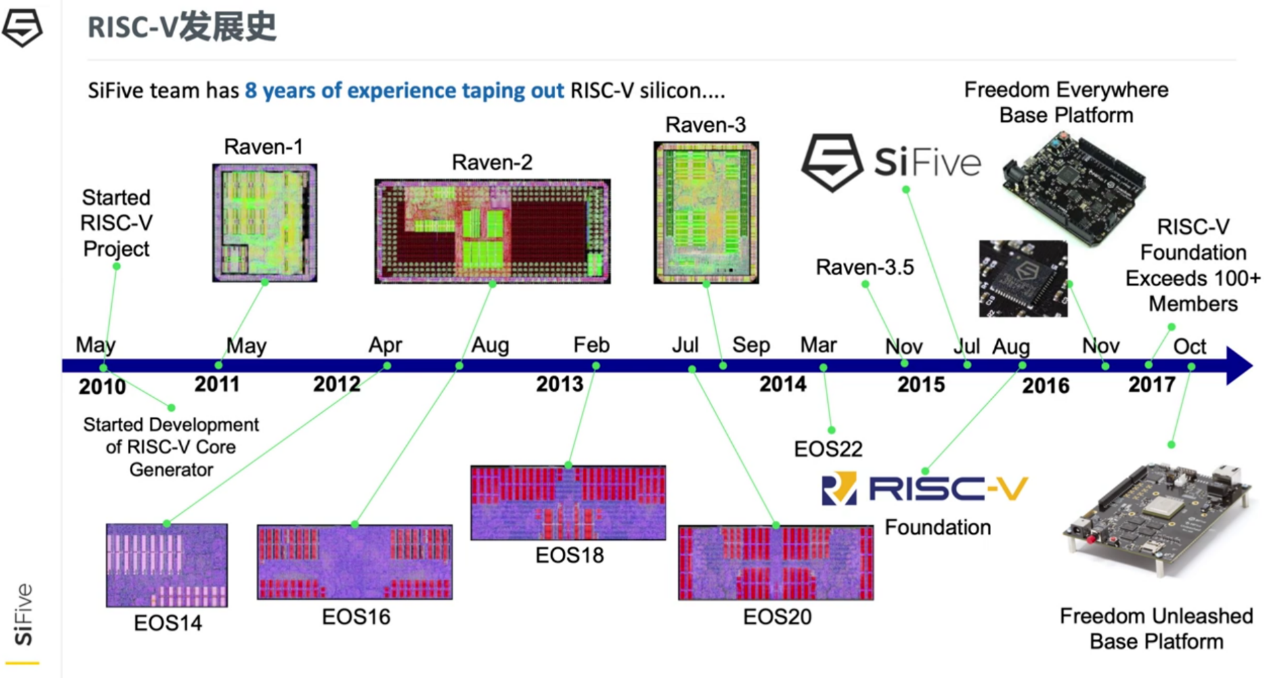
\includegraphics[scale=0.8]{img/one.png}
				\end{figure}
			\subsubsection{RISC-V指令结构}
				\begin{enumerate}
					\item 
						RSICV指令集分为基本指令集I和扩展指令集M,A,F,D,C。基本指令集I是整数指令集,也是RISC-V中,对于任何处理器必须有的指令集,扩展指令集可有可无。
					\item
						基本指令集有六种格式:
					\begin{enumerate}		
						\item 
							R 类型指令:用于寄存器 - 寄存器操作;
						\item 
							I 类型指令:用于短立即数和访存 load 操作;
						\item 
							S 类型指令:用于访存 store 操作;
						\item 
							B 类型指令:用于条件跳转操作;
						\item 
							U 类型指令:用于长立即数操作;
						\item 
							J 类型指令:用于无条件操作;
					\end{enumerate}
					\begin{figure}[!htbp]
						\centering
						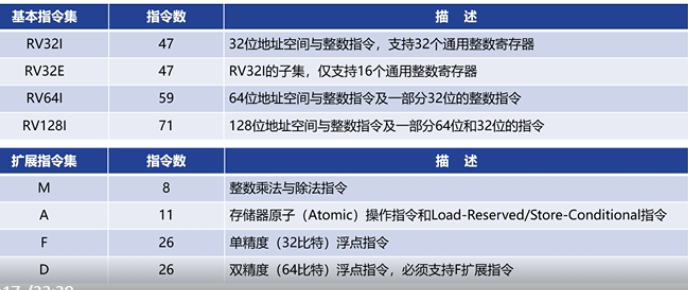
\includegraphics[scale=0.8]{img/two.png}
					\end{figure}
					\begin{figure}[!htbp]
						\centering
						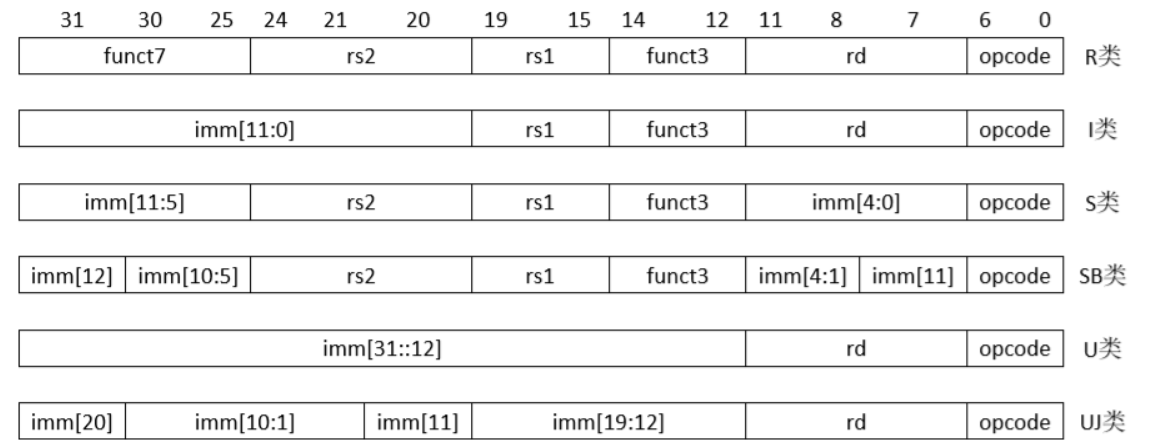
\includegraphics[scale=0.5]{img/three.png}
					\end{figure}
				\end{enumerate}

		\subsection{蜂鸟E203简介}
			\subsubsection{E203}
				\begin{enumerate}
					\item 
						蜂鸟 E203 系列处理器由作者所在的公司开发,是一款开源的 RISC-V 处理器。蜂鸟是世
						界上最小的鸟类,其体积虽小,却有着极高的速度与敏锐度,可以说是“能效比”最高的鸟类。
						E203 系列以蜂鸟命名便寓意于此,旨在将其打造成为一款世界上最高能效比的 RISC 处理器。
				\end{enumerate}	
				\begin{figure}[!htbp]
					\centering
					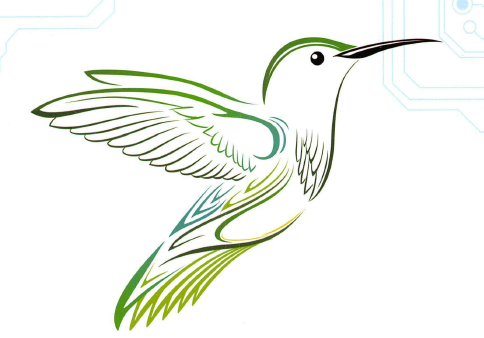
\includegraphics[scale=0.8]{img/four.png}
				\end{figure}
					
			\subsubsection{E203 核心数据通路的模块划分}
				\begin{enumerate}
					\item 
						IFU 取址单元
					\item 
						EXU 执行单元
					\item 
						LSU 访存单元
					\item 
						BIU 总线
				\end{enumerate}	

			\subsubsection{E203 数据通路的两级流程水线}
				\begin{enumerate}
					\item 
						第一级是IFU,包括,取址、分支预测、生成PC。
					\item 
						第二级是译码、派遣、执行、访存、写回。
				\end{enumerate}	

			\subsubsection{E203 的特点}
				\begin{enumerate}
					\item 
						蜂鸟E203 处理器研发团队拥有在国际一流公司多年开发处理器的经验,使用稳健的。
					\item 
						蜂鸟E203 的代码为人工编写,添加丰富的注释且可读性强,非常易于理解。
					\item 
						蜂鸟E203 专为IoT 领域量身定做,其具有2 级流水线深度,功耗和性能指标均优于目前主流商用的ARM Cortex-M 系列处理器,且免费开源,能够在IoT 领域完美替代ARM Cortex-M 处理器。
				\end{enumerate}	

		\subsection{T-core开发板介绍}
			\begin{enumerate}
				\item 
					T-core开发板是友晶科技公司的基于RISC-V的新款开发板。T-Core提供了围绕Intel MAX 10 FPGA构建的强大的硬件设计平台。它配备完善,可在控制平面或数据路径应用中提供具有成本效益的单芯片解决方案,并提供行业领先的可编程逻辑,以实现最终的设计灵活性。
				\item 
					借助MAX 10 FPGA,可以获得比上一代更低的功耗/成本和更高的性能。可支持大量应用,包括协议桥接,电机控制驱动,模数转换和手持设备。T-Core开发板包括硬件,例如板载USB-Blaster II,QSPI Flash,ADC接头连接器,WS2812B RGB LED和2x6 TMD扩展接头连接器。通过利用所有这些功能,T-Core是展示,评估和原型化Intel MAX 10 FPGA真正潜力的理想解决方案。T-Core还通过板载JTAG调试支持RISC-V CPU。它是学习RISC-V CPU设计或嵌入式系统设计的理想平台。
			\end{enumerate}	
			\begin{figure}[!htbp]
				\centering
				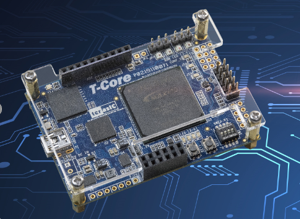
\includegraphics[scale=1]{img/five.png}
			\end{figure}
			\begin{figure}[!htbp]
				\centering
				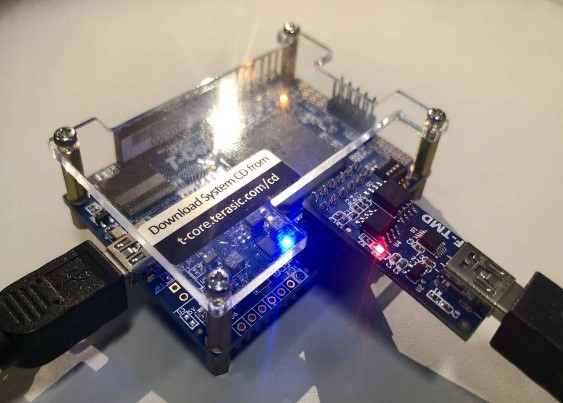
\includegraphics[scale=1]{img/six.jpg}
			\end{figure}

	\section{实践篇}
	
	\begin{figure}[H]
		\centering  
		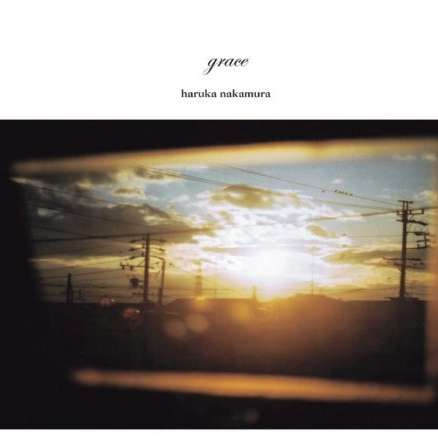
\includegraphics[scale=0.7]{img/avatar.jpg}   
		\caption{DHCP Request包字节形式}
	\end{figure}

	\begin{enumerate}
		\item 
	\end{enumerate}

	\begin{itemize}
		\item 
	\end{itemize}

	\begin{lstlisting}[language={C++}]
	class Pokemon : public QObject  	//代码
	\end{lstlisting}
	
	\begin{table}[H]
		\centering
		\begin{tabular}{lll}
			\hline
			字段 & 值 & 含义 \\ \hline
			包头长度 & 45 & 数据分组首部长度20字节 \\ \hline
			服务类型 & 00 & 正常时延、正常吞吐量、正常可靠性 \\ \hline
			总长度 & 003c & 数据分组长度60字节 \\ \hline
			标识 & 5c6e & 标识为23662 \\ \hline
			标志 & 00 & MF=0:此片为最后一片,DF=0:允许分片 \\ \hline
			片偏移 & 00 & 偏移量=0 \\ \hline
			TTL & 40 & 每跳生存周期为64 \\ \hline
			协议 & 01 & 来自ICMP协议 \\ \hline
			头部校验和 & 0000 & IP头部检验和为0000 \\ \hline
			源地址 & c0a86386 & 源地址为192.168.99.134 \\ \hline
			目的地址 & 72ff28a6 & 目的地址为114.255.40.166 \\ \hline
		\end{tabular}
	\end{table}
	
	\section{结果展示}
	
	\section{未来展望}
	
\end{document}